\chapter{Evaluation}
\label{chapter:evaluation}

%This will cover the setup I used to record data.  Here is gets a little dicey with respect to not disclosing information about the car.  I plan to handle this by talking to the full extent about my cameras only.  I only use other sensors for groundtruth so it doesn't need to be covered in detail.  I will cover it at a very high level e.g. 'High Accuracy GPS with x cm accuarcy'.  Check with Jan about this.

\section{Hardware Setup}

\subsection{Platform}

A vehicle was used to do the recording.  The vehicle was equipped with GPS and inertial sensors for collecting ground truth data.  A computer with a RAID array was used to record all relevant data.  ROS was used to synchronise and record the data.  Although ScaViSLAM is capable of almost real time processing, processing was done offline with playback slowed to half speed.

The computer used for processing was a Intel Xeon 3.2Ghz quad core with 12Gb of memory and a Quadro 2000 graphics card.  ScaViSLAM, place recognition and the loop closure pipeline all run simultaneously in separate threads.

\subsection{Cameras}

\subsubsection{Stereo Camera}

For the stereo camera, a Bosch\footnote{\url{http://www.bosch-automotivetechnology.com/}} Stereo Video Camera (SVC)was used.  This is a stereo camera designed for automotive use and therefore has a casing that fits well to the inside of a car windshield.  (See Fig. \ref{fig:bosch_svc})

Multiple cameras were evaluated with ScaViSLAM in an outdoor setting, including a Point Grey\footnote{\url{http://ww2.ptgrey.com/stereo-vision/bumblebee-2}} Bumblebee 2 and a Videre \footnote{\url{http://users.rcn.com/mclaughl.dnai/}} STH-DCSG-VAR.  The Bosch SVC was choosen as it showed to have the best image quality and shutter/gain control in outdoor conditions, where the sun would sometimes shine directly into the lense.  The SVC has an additional feature of being able to calculate an extrinsic calibration online with respect to the vehicle's base coordinate frame.  This is useful for calibration to the vehicle's ground truth data.

The stereo camera has a baseline of 12cm.  The each video camera has a resolution of 1024x512 pixels, outputs grey scale images with 8 bit pixel depth and a framerate of 15fps.  The frontend of ScaViSLAM uses dense stereo tracking on the GPU, which scales very poorly to high resolution imagery and therefore the images were scaled down to 512x256 pixels for the frontend tracking, however for the place recognition and loop closure pipeline the original image was used.

\begin{figure}[h]
  \centering
    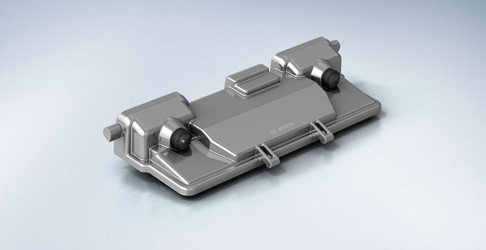
\includegraphics[width=0.7\textwidth]{chapters/images/svc}
  \caption{Bosch stereo camera}
  \label{fig:bosch_svc}
\end{figure}

\subsubsection{Omni Camera}

The omni camera used for evaluation was an Allied Vision Technologies\footnote{\url{http://www.alliedvisiontec.com}} (AVT) Stingray camera, paired with a Palnon\footnote{\url{http://www.tateyama.jp/eng/}} omni directional lense.  For the experiments performed, 1280x960 pixel images with 8 bit depth were recorded at 30fps.  

The AVT camera is a generic camera, not specifically designed for omni-directional lenses and operates over a standard firewire 1394 interface.  As a result, the shutter and gain controls needed to be changed to ignore areas of the donut image with no data.  In this case the camera driver\footnote{ROS camera1394 package, \url{http://wiki.ros.org/camera1394}} was modified so that the calculation of the image brightness only considered valid pixels.

%These images were unwrapped to the circular images with a resolution of 2547x405.

\begin{figure}[h]
  \centering
    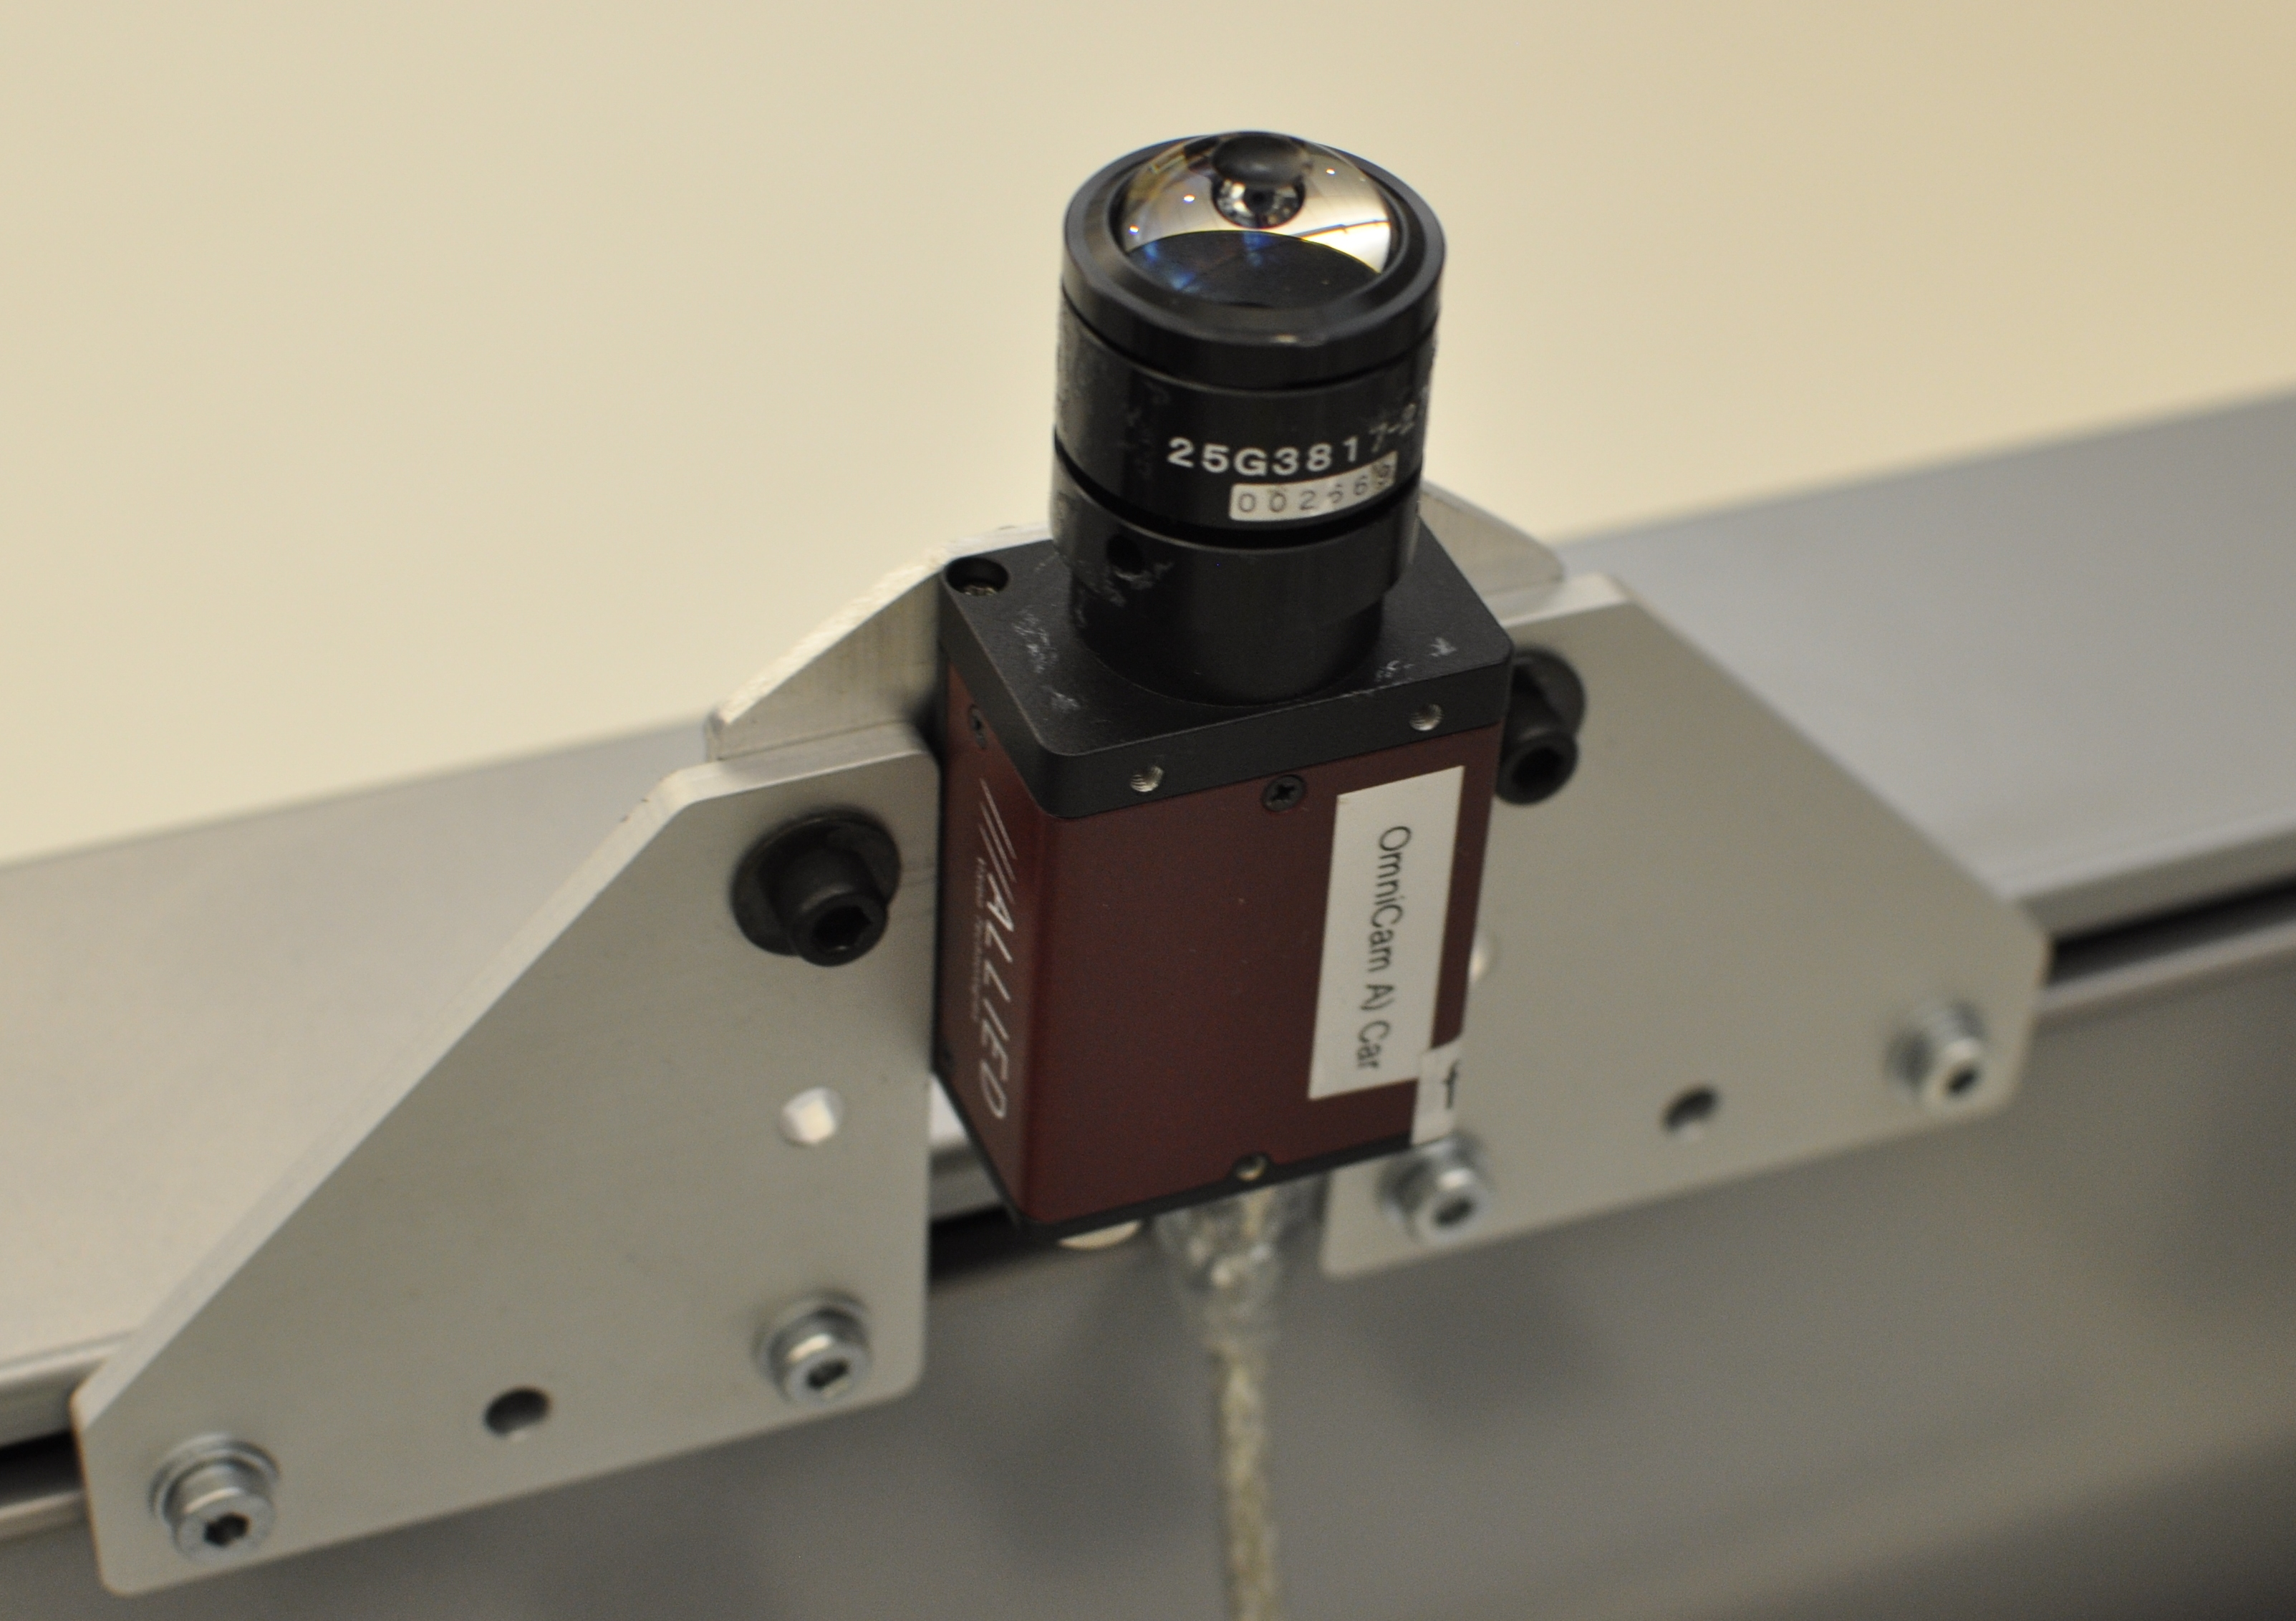
\includegraphics[width=0.5\textwidth]{chapters/images/omni_cam_image}
  \caption{AVT camera with the omni-directional lense and mounting brackets attached}
\end{figure}

\subsubsection{Camera Calibration}

Theory behind all the algorithms used is explained in Chapter \ref{chapter:extrinsic_calibration}, this section will describe the procedure undertaken.  The first step involved using the ROS calibration tool described in Section \ref{sec:ros_tool}.  This tool requires no initial condition to determine a calibration.  This was performed indoor with a checkerboard, but produced poor results because of the limited room to move the checkerboard around.

The calibration from the ROS calibration was used as an initial condition for the non linear optimization refinement. (See Section \ref{sec:g2o_extrinsic_cal}).  Video data was recorded outside using the online verification tool \ref{sec:verification_tool}.  In order to collect points of different depth, a textured surface was held in front of the camera at close range and moved slowly away.  Being outside, many distant points were also recorded.  The non linear extrinsic refinement tool was then run to obtain a refined calibration.   

\subsection{Groundtruth}

A combination of Differential Global Positional System (DGPS) and inertial sensors provided a ground truth trajectory poses (translation and rotation) with an accuracy of less than 50cm. 

\section{Evaluation Method}

The RGBD dataset tools\cite{sturm12iros} were used in order to evaluate error metrics on the trajectories generated by the modified ScaViSLAM system.  The RGBD dataset tools provide two metrics for evaluating trajectories; Absolute Trajectory Error (ATE) and Relative Pose Error (RPE).

\subsubsection{Relative Pose Error}

RPE is a measure of trajectory accuracy over some small fixed time interval.  In that sense it is a measure of drift.  If a trajectory to be evaluated is defined as $\bv P_1,....,\bv P_n \in \text{SE}(3)$ and the ground truth as $\bv Q_1,....,\bv Q_n \in \text{SE}(3)$ then the RPE at timestep $i$ may be defined as:

\begin{equation}
 \bv E_i := (\bv Q_i^{-1} \bv Q_{i+\Delta})^{-1}(\bv P_i^{-1} \bv P_{i+\Delta})
\end{equation}

The final root mean squared error (RMSE) over all time steps can be evaluated as:

\begin{equation}
 \text{RMSE}(\bv E_{1:n}) := \left( \dfrac{1}{m}\displaystyle\sum\limits_{i=1}^m \| trans(\bv E_i) \| ^2 \right)^\frac{1}{2}
 \label{eq:rmse}
\end{equation}

$trans()$ is a function taking only the translation component of the error and $m$ is total number all time intervals for a sequence of $n$ camera poses. 

This is a measure of drift, and is more applicable to visual odometry systems.  In this case the final SLAM graph trajectory after loop closures is of interest to us, not the visual odometry drift.  Loop closures should have little affect on the amount of drift in the SLAM system and therefore this method will not be used.

\subsubsection{Absolute Trajectory Error}

Absolute Trajectory Error evaluates how well an entire trajectory aligns to another one.  In order to compute this metric, first the trajectories need to be aligned as best as possible.  Horn\cite{Horn87} provides a closed form function to find the rigid body transformation $\bv S$ that performs this alignment of trajectory $\bv P$ onto ground truth trajectory $\bv Q$.  The error can then be computed for time step $i$ as follows:

\begin{equation}
 \bv E_i := \bv Q_i^{-1}\bv S \bv P_i
\end{equation}

The total RMSE can then be computed as per eq. \ref{eq:rmse}

The ATE provides a good measure of complete trajectory accuracy and therefore should be able to indicate if the loop closures provide an overall improvement to a trajectory.

\section{Experiments}

%\subsection{Data Collection Area}

%For all data to be evaluated, a car park was choosen.

\subsection{Routes}

Two routes were selected for the evaluation.  The first 'two loops' dataset involved driving a small loop around two buildings, doing a three point turn, and then traversing the loop backwards to the start.  The idea behind this dataset is to provide ideal conditions to demonstrate the improvement that omni-loop-closures may bring.  There are no overlapping sections of this trajectory where the car has the same pose on first and second visit, therefore the original stereo only system should not find any loop closures.

The second route 'car park loops', involves driving loops around 3 buildings and part of a car park.  This is a longer, more realistic sequence which should allow a more fair comparison of the original system with the omni-loop-closure version.

\begin{figure}[h]
  \centering
    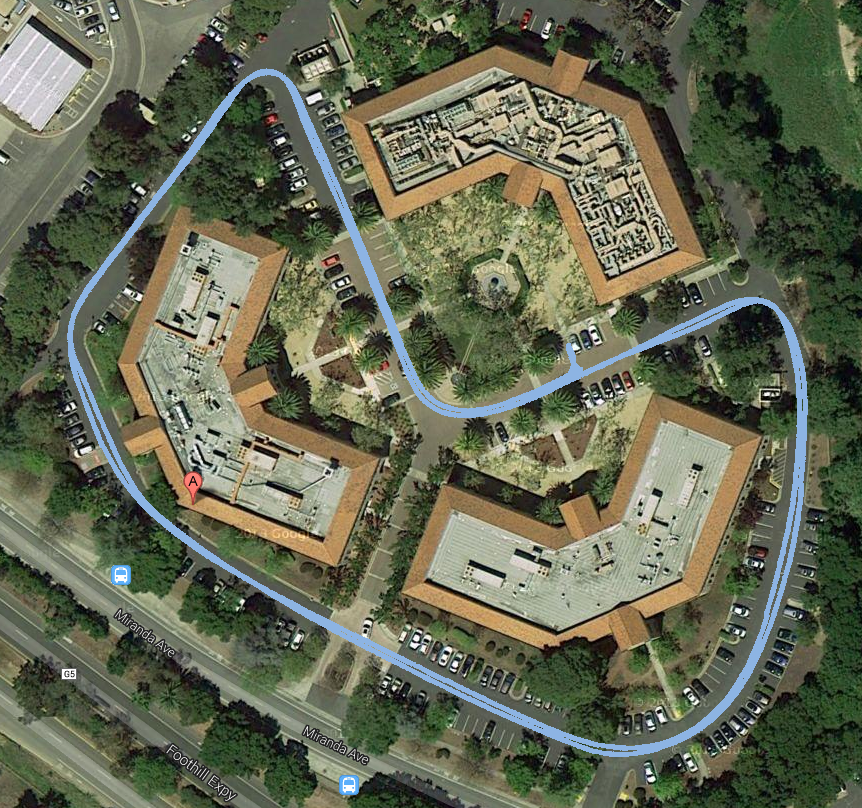
\includegraphics[width=0.553\textwidth]{chapters/images/two_loops_overlay}
    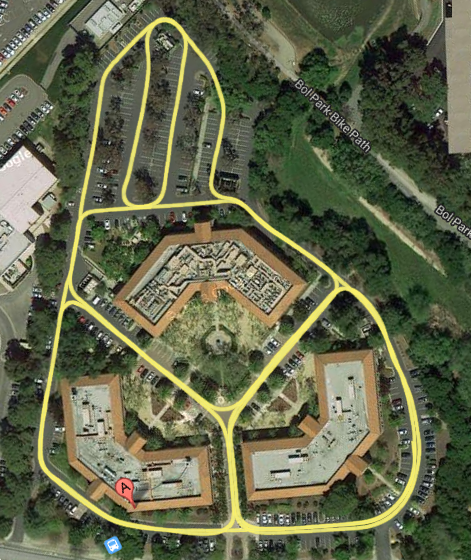
\includegraphics[width=0.437\textwidth]{chapters/images/carpark_loops_overlay}
  \caption{Overlay of the GPS ground truth on satellite imagery for both routes}
\end{figure}

\begin{table}[h]
    \begin{tabular}{ p{8.5cm} r r} % p{5cm} |}
    \toprule
    & Two loops & Carpark loops \\
    \midrule
    Total Distance & 1132m & 2167m \\
    Overlapping distance (driving in either direction)& 553m & 1085m \\
    Overlapping distance (driving the same direction)& 0m & 655m \\
    Average Speed & 4.43 m/s & 5.12 m/s \\
    Time & 4:12s & 7:03s \\
    \bottomrule
    \end{tabular}
    \captionof{table}{Statistics on the two datasets recorded}
  \label{tab:geometry}
\end{table}

\subsubsection{Driving conditions}

'Two loops' was recorded during the middle of the day, with little traffic and very good weather conditions.  It is meant to be the most ideal conditions for the algorithm.  On the other hand car park loops was recorded in the morning when the sun was low in the sky.  This often created lense flare in both cameras, and therefore introduced some interference to the algorithms.  The reasoning behind recording such a sequence is to show that not only is the loop closure pipeline robust in non ideal conditions, but also that it can provide significant benefits where visual odometry may fail.

\begin{figure}[h]
  \centering
    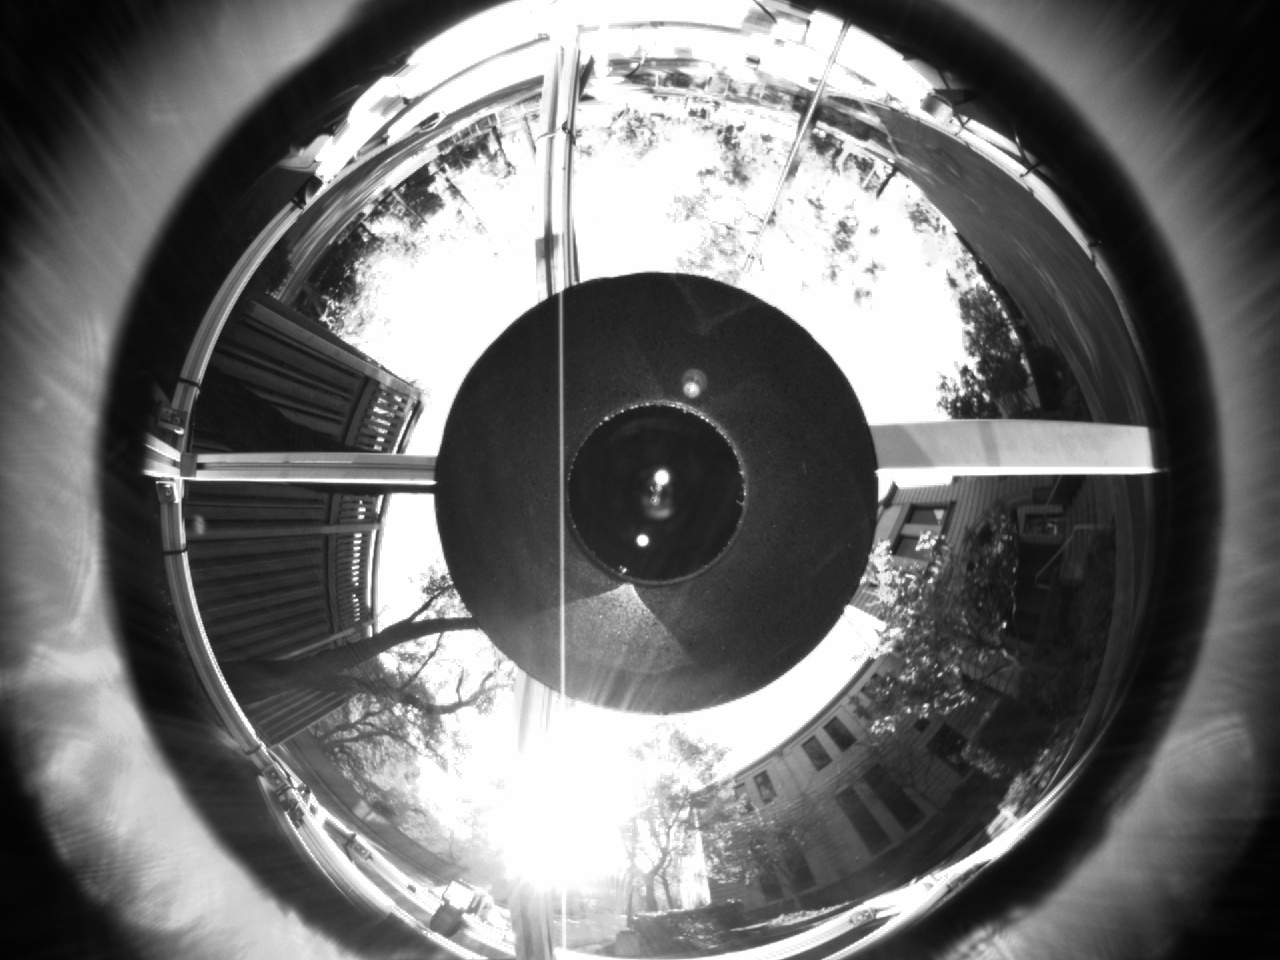
\includegraphics[width=0.40\textwidth]{chapters/images/omni_lense_flare}
    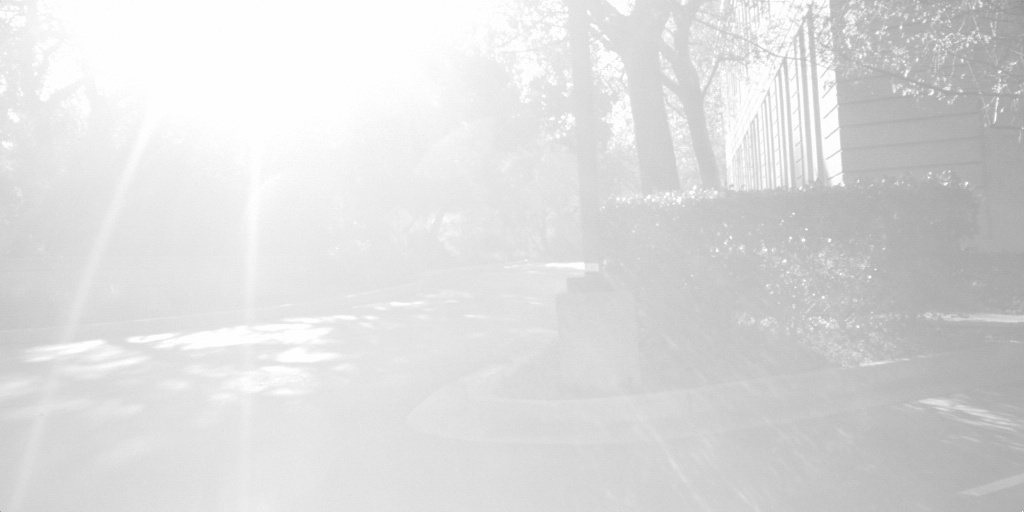
\includegraphics[width=0.59\textwidth]{chapters/images/stereo_lense_flare_bad}
  \caption{Example of lense flare in 'car park loops' dataset}
\end{figure}

\subsection{Quantitative evaluation}

It is clear from Table \ref{tab:ate_results} that the omni loop closure pipeline clearly outperforms the original ScaViSLAM algorithm in both datasets.  Comparing only the RMSE values, the omni loop closure pipeline provided a 82.4\% and 50.2\% improvement in accuracy on the two loop and car park loop datasets respectively. 

\begin{table}[h]
  \centering
    \begin{tabular}{ p{5cm} r r r r} % p{5cm} |}
    \toprule
    & \multicolumn{2}{c}{\bf{Two loops}}  & \multicolumn{2}{c}{\bf{Carpark loops}} \\
    & Stereo & Omni & Stereo & Omni \\
    \midrule
    RMSE              & 23.748 & 4.172 & 20.067  &  9.995 \\
    Standard deviation& 6.374  & 1.899 & 9.591   &  5.768 \\
    Min Error         & 8.815  & 0.343 & 1.819   &  0.816 \\
    Max Error         & 34.161 & 8.681 & 55.674  & 51.626 \\
    \bottomrule
    \end{tabular}
    \captionof{table}{Absolute Trajectory Error results.  All units are in meters. Stereo denotes only stereo for loop closures, omni denotes the loop closure pipeline}
  \label{tab:ate_results}
\end{table}

Take note of the large maximum error for both systems on the car park loops dataset.  This is due to the fact that tracking was lost for a short period of time before ScaViSLAM recovered.  In both cases a keyframe at the point before the tracking dropout occured was moved to the location where tracking recovered from graph optimization.  

\begin{figure}[h]
  \centering
    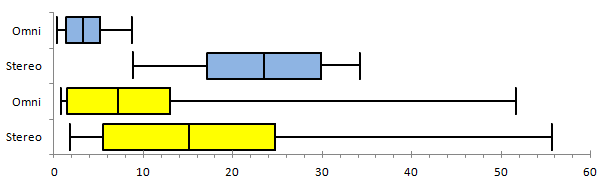
\includegraphics[width=1.00\textwidth]{chapters/images/box}
  \caption{Box plot of results.  Blue denotes the two loops sequence and yellow denotes the car park loops sequence}
  \label{fig:box_plot}
\end{figure}

Fig. \ref{fig:box_plot} visualizes the data in Table \ref{tab:ate_results}, showing median, standard deviation, min and max values.  This makes the reduction in error for both datasets very visible.  For the two loops sequence, one can clearly see that the maximum error of the omni-loop-closure system is the same as the minimum error for the original system.  

\subsection{Qualitative evaluation}

Fig. \ref{fig:two_loops_quantitative} illustrates the SLAM graphs for the two loops dataset.  The omni-loop-closures are visible top right between the two loops, and have occurred almost throughout the entire loop. 

\begin{figure}[h]
  \centering
    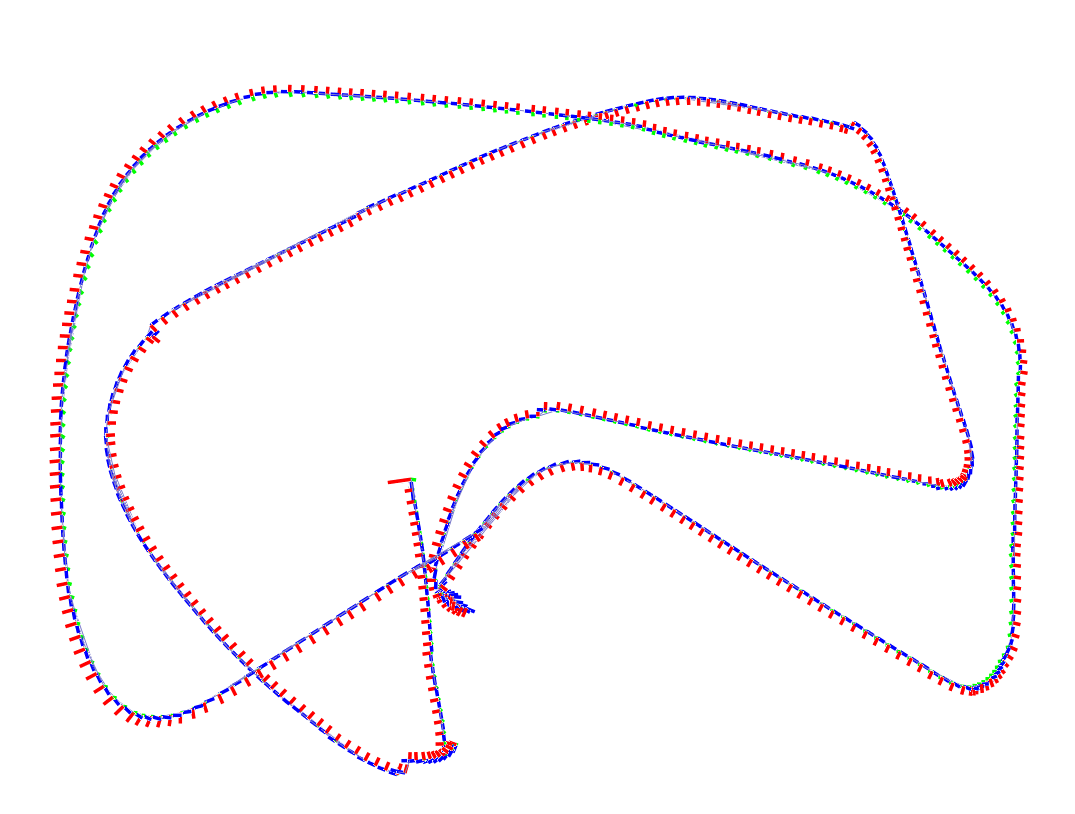
\includegraphics[width=0.49\textwidth]{chapters/images/stereo_above}
    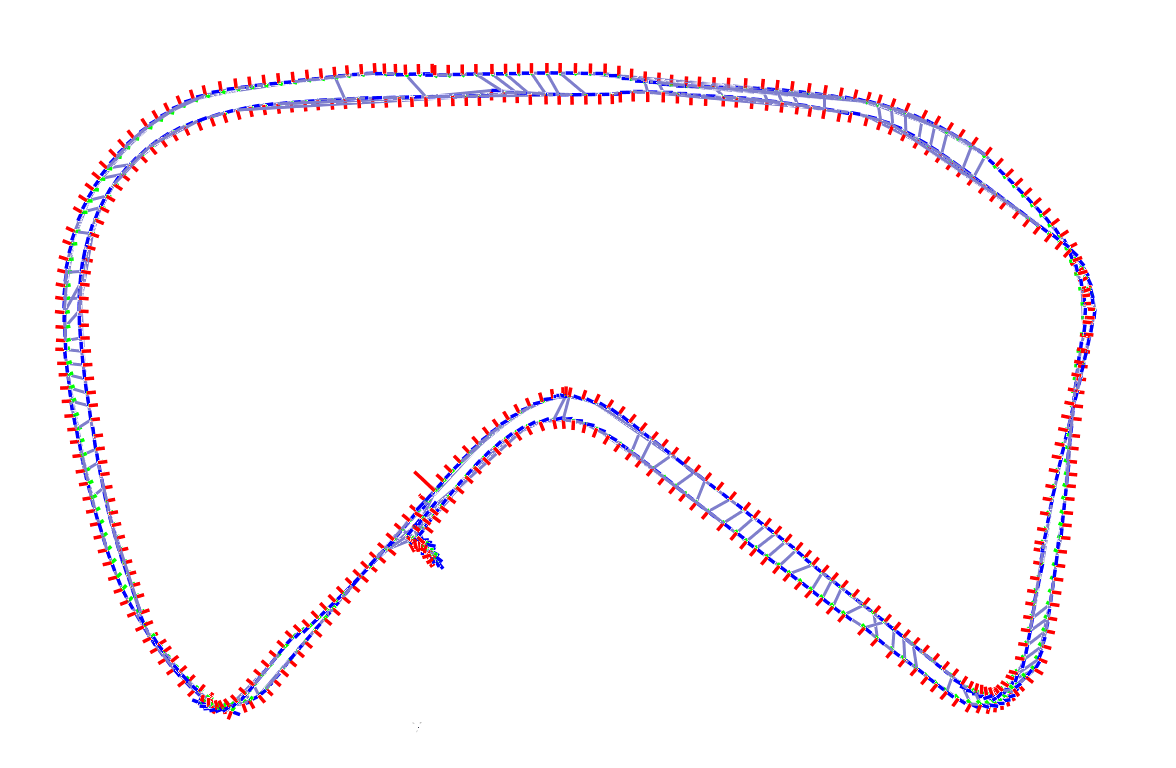
\includegraphics[width=0.49\textwidth]{chapters/images/omni_above}\\
    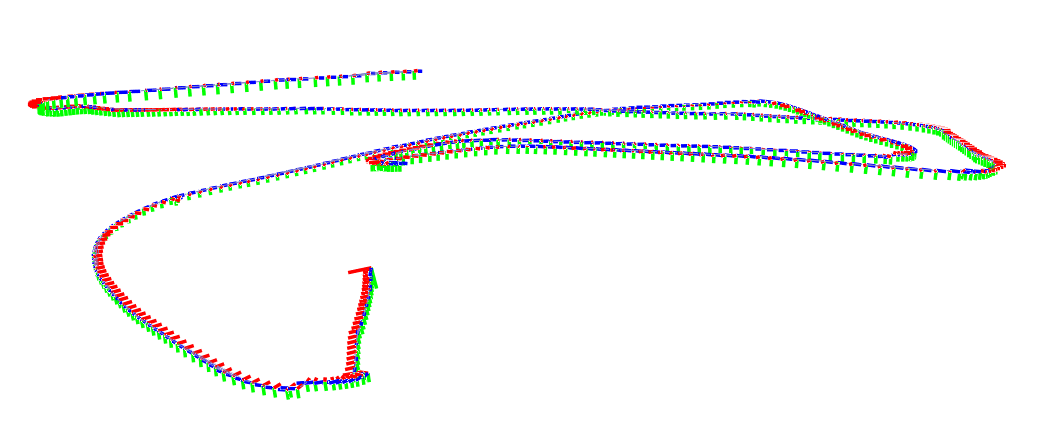
\includegraphics[width=0.49\textwidth]{chapters/images/stereo_side}
    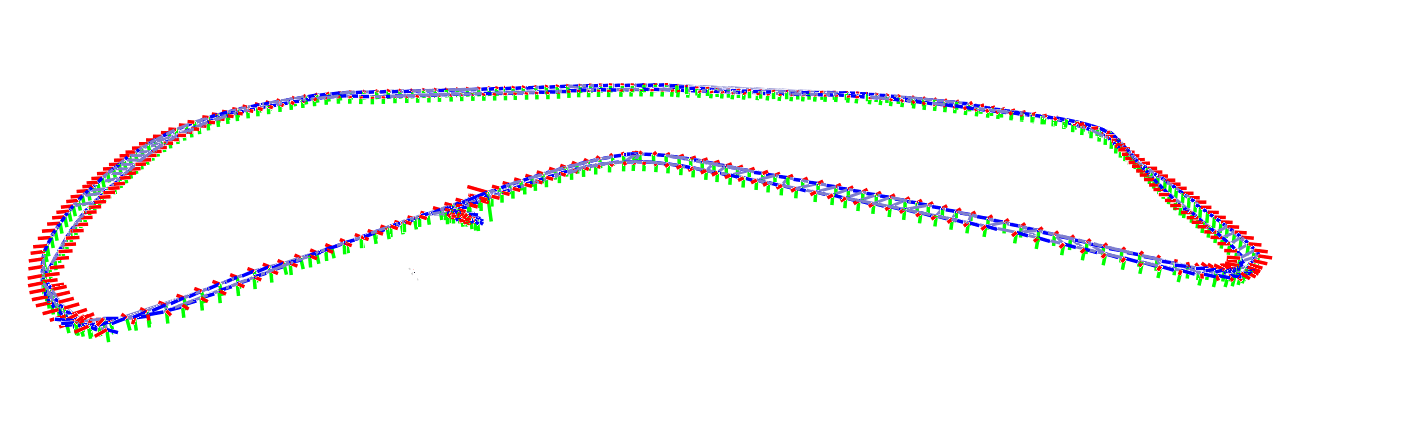
\includegraphics[width=0.49\textwidth]{chapters/images/omni_side}
  \caption{SLAM graphs comparison for 'two loops' dataset.  Left shows the original ScaViSLAM system and right is the system with omni-loop-closures}
  \label{fig:two_loops_quantitative}
\end{figure}

As expected, there were no large loop closures for the stereo only version, and therefore the drift propagated throughout the entire trajectory.  There was clearly some error in the visual odometry during the three point turn between loops which caused an incorrect heading as the vehicle started the second loop, hence why the second loop is so poorly misaligned with the first one.

Inspecting the stereo only system there was clearly a significant amount of drift upward with respect to the road that occurred during the entire sequence.  This drift appears to be completely corrected by the omni-loop-closures.


\begin{figure}[h]
  \centering
    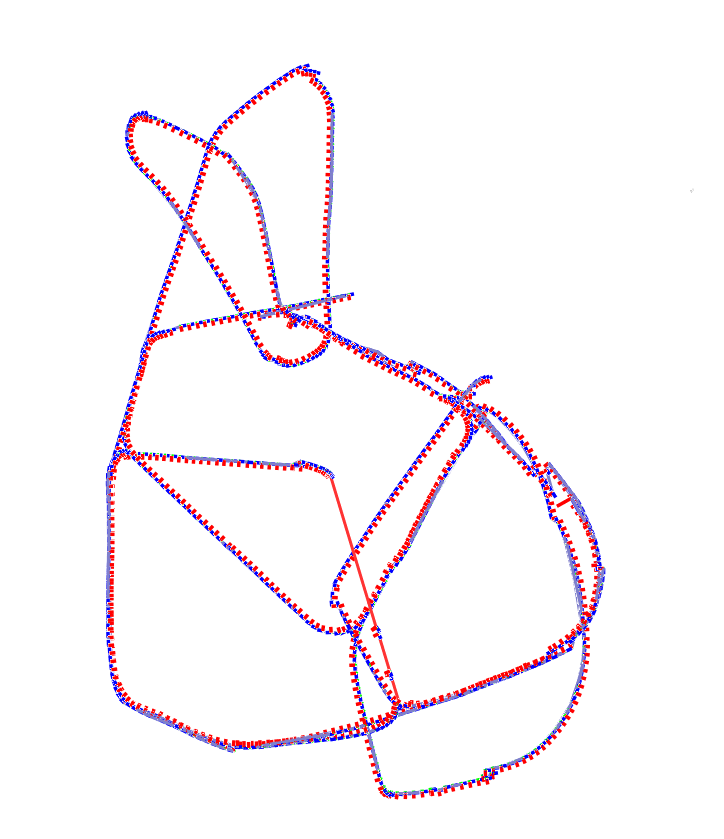
\includegraphics[width=0.49\textwidth]{chapters/images/stereo_above_carpark}
    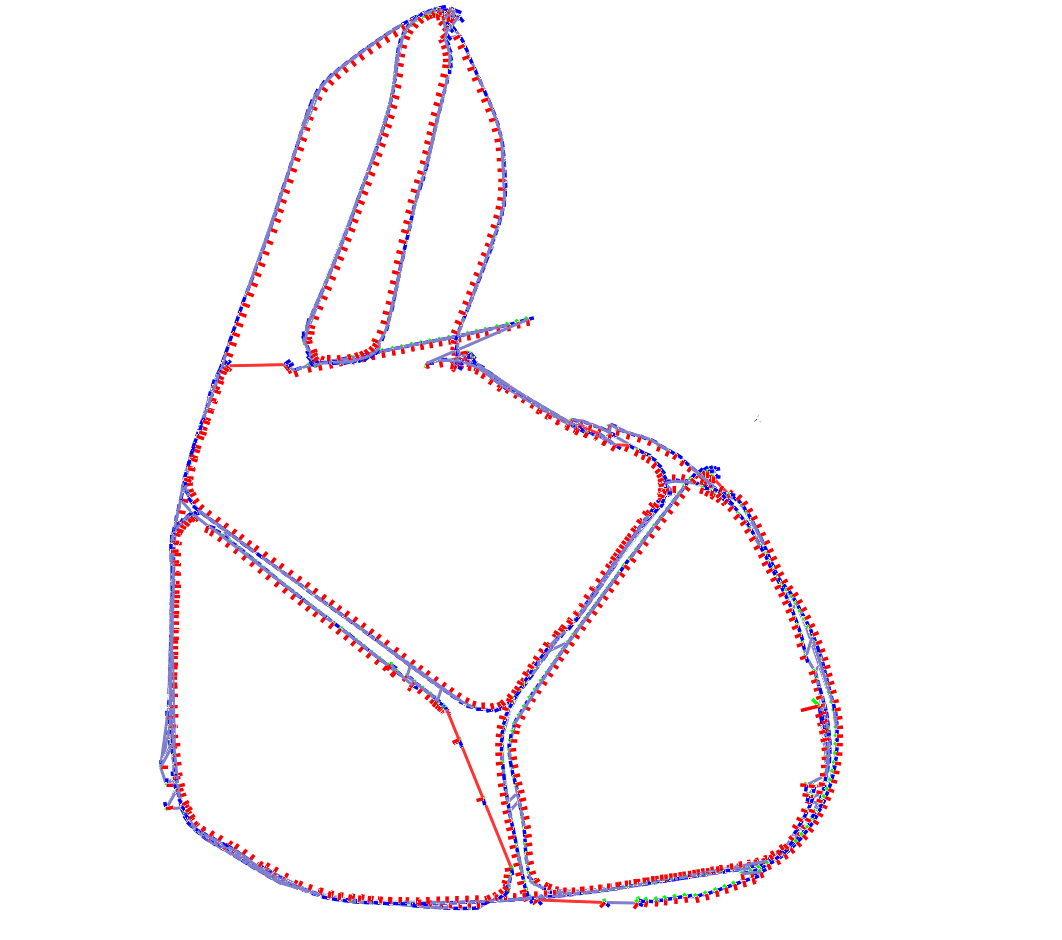
\includegraphics[width=0.49\textwidth]{chapters/images/omni_above_carpark}\\
    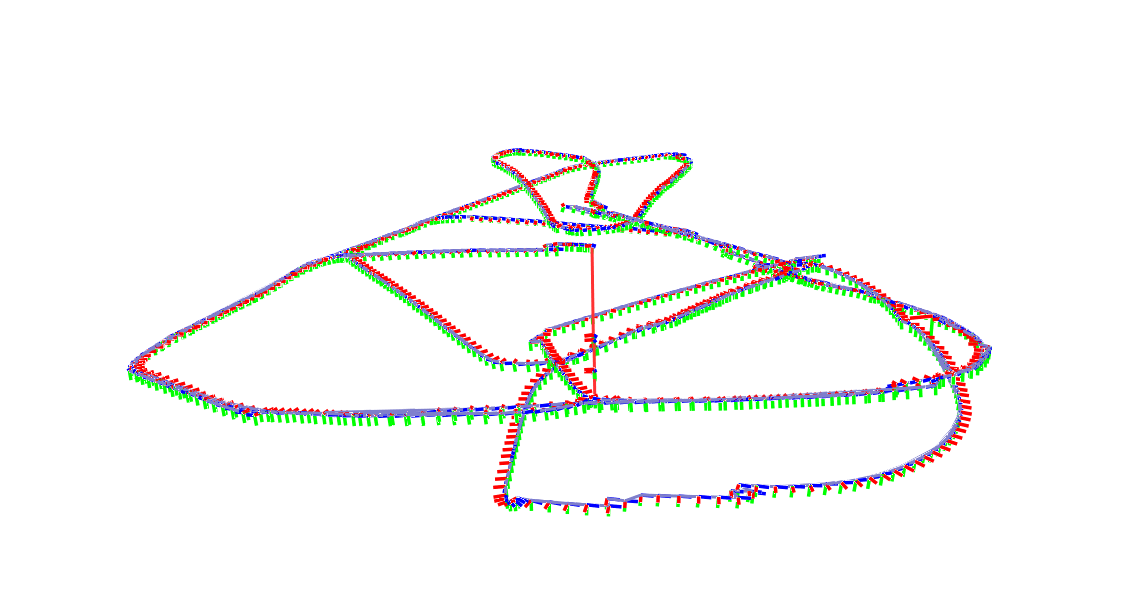
\includegraphics[width=0.49\textwidth]{chapters/images/stereo_side_carpark}
    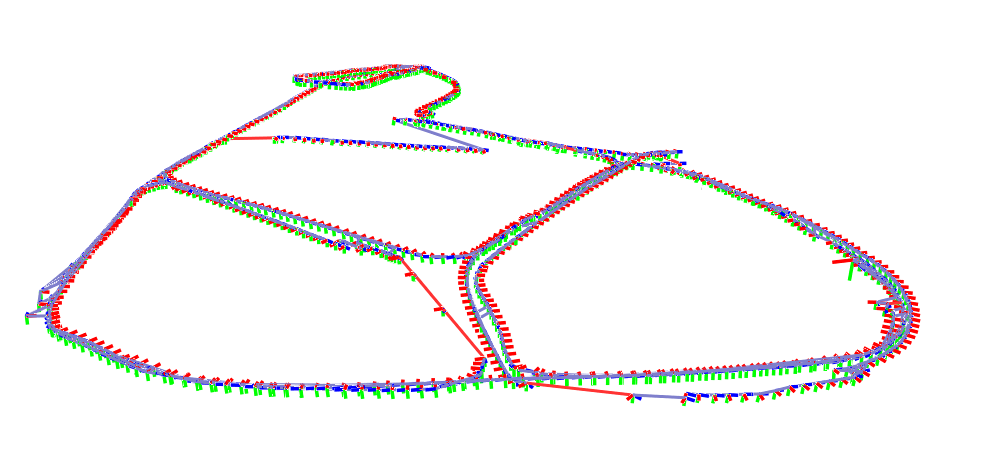
\includegraphics[width=0.49\textwidth]{chapters/images/omni_side_carpark}
  \caption{SLAM graphs comparison for 'car park loops' dataset.  Left shows the original ScaViSLAM system and right is the system with omni-loop-closures}
  \label{fig:carpark_loops_quantitative}
\end{figure}

Fig. \ref{fig:carpark_loops_quantitative} shows the comparison for the car park loops dataset.  It is clear to see that the omni-loop-closure pipeline resulted in a much more consistent and accurate trajectory.

It is important to point out that tracking was lost in during this sequence for a short period in both systems due to the sun shining directly into the stereo camera.  This is visible in both SLAM graphs as a long red line separating the two bottom buildings.  Whilst both systems recovered tracking and restored the correct pose via a loop closure, the stereo only system clearly failed to retain a consistent graph.  On the other hand the omni-loop-closure pipeline was able to make an opposite direction loop closure on the section of road preceding the tracking failure and the erroneous edges are correctly stretched where keyframes are missing.

Another significant source of error in the stereo only system is the unaligned loop for the bottom right building.  Again, this was correctly aligned in the omni-loop-closure case via an opposite direction loop closure.

An important observation from both datasets is that although there are many instances of omni-loop-closures, they did not consistently occur everywhere in overlapping sections of the trajectories.  This would have been expected especially for the two loops dataset, which had ideal conditions for the omni-loop-closure pipeline.  This will be examined in more detail in the next section.

\subsection{Loop Closure Statistics}

Table \ref{tab:place_recog_stats} shows the place recognition statistics for 'two loops' dataset.  This is also visualized in \ref{fig:place_recog_stats}.  It is clear that many of the loop closures are outliers, only 18\% were valid results.  Nevertheless the geometry check rejected all false negatives allowing only valid loop closures to be added to the graph.

\begin{table}[h]
  \centering
    \begin{tabular}{ p{5cm} r r} % p{5cm} |}
    \toprule
    & Number of Loop Closures & Percent \\
    \midrule
    Total processed           & 2125 & 100\% \\
    Keyframes with matches    & 275  & 12.9\% \\
    Successful loop closures  & 118  & 5.5\% \\
    \bottomrule
    \end{tabular}
    \captionof{table}{Loop closure statistics for two loops dataset.  Total attempted is all loop closures checked by the loop closure pipeline.  Keyframes with matches are keyframe pairs that had successfully matched the omni camera images, but failed due to not enough triangulated points or not enough scale offset points}
  \label{tab:place_recog_stats}
\end{table}

The left image in \ref{fig:place_recog_stats} shows that some of the keyframes have many more edges than others.  This means that the place recognition module had a bias for certain keyframes.  For most of the route, there is building on one side of the car, and trees on the other.  In addition the two buildings have almost identical facades.  Therefore some parts of the route are rather indistinctive and the place recognize is likely matching similar looking parts of the buildings.

The center image \ref{fig:place_recog_stats} is also of interest.  There are sections of the track where there are no failed loop closures.  This means that these pairs were either not identified as loop closure candidates at all.  It also shows many red links between the two loops.  In this case the loop closures failed due to lack of points used for pose estimation, or there were not enough circular matches to calculate scale offsets.  Stereo features need to be matched with features used in the omni images for pose estimation.  As the field of view of the stereo camera is limited, it is very conceivable that sometimes no matches would exist.

\begin{figure}[h]
  \centering
    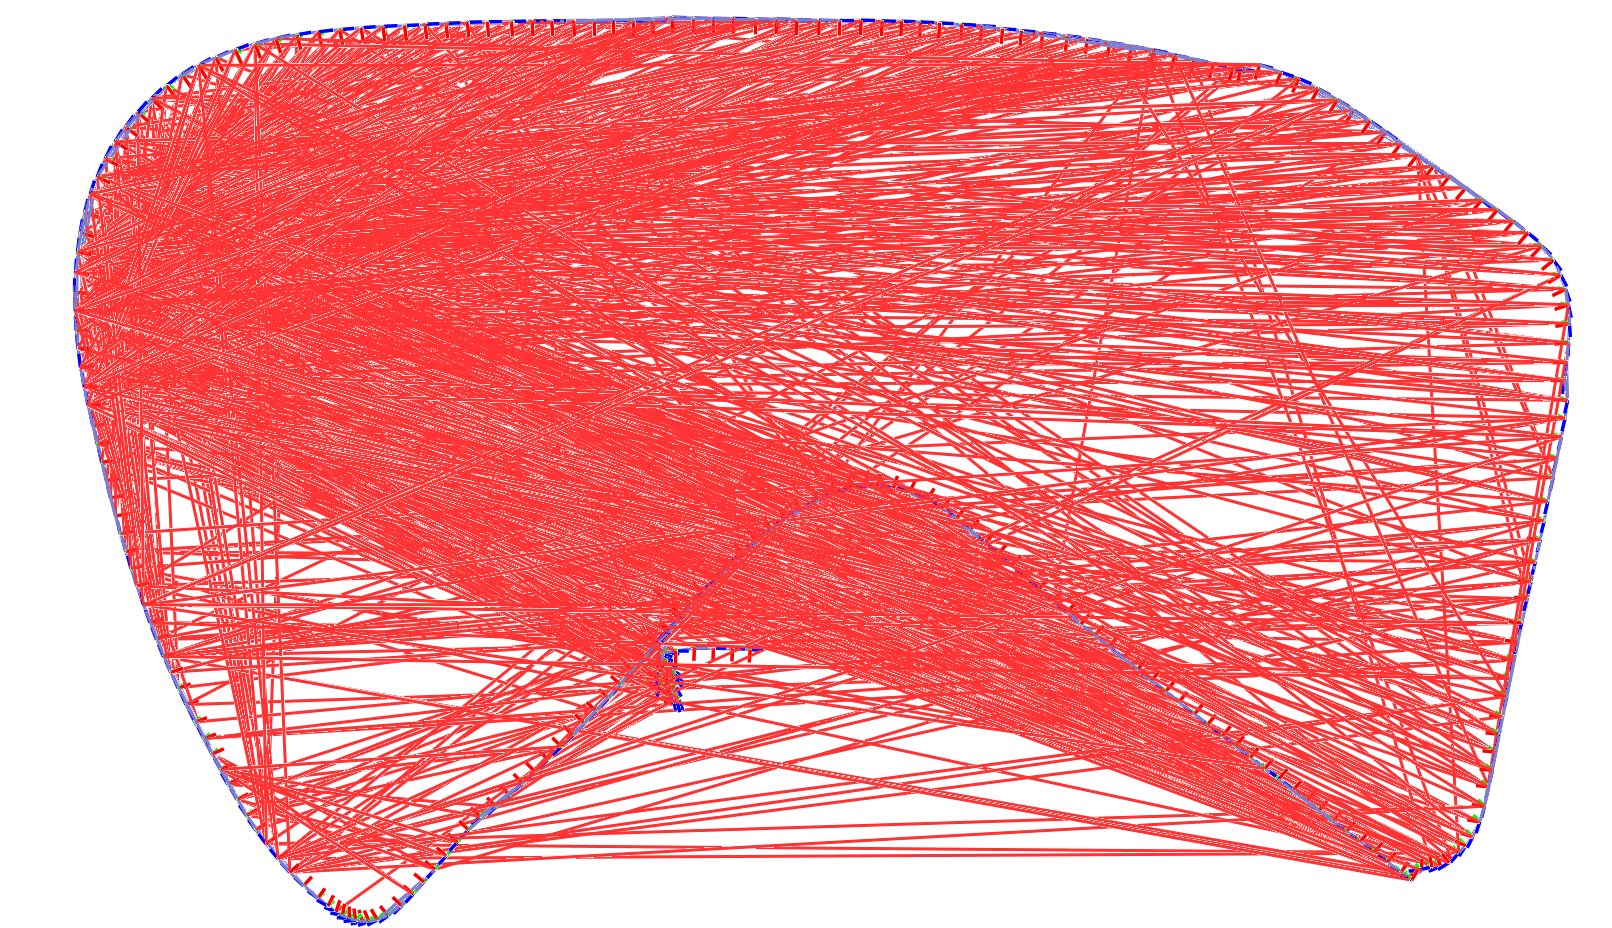
\includegraphics[width=0.32\textwidth]{chapters/images/all}
    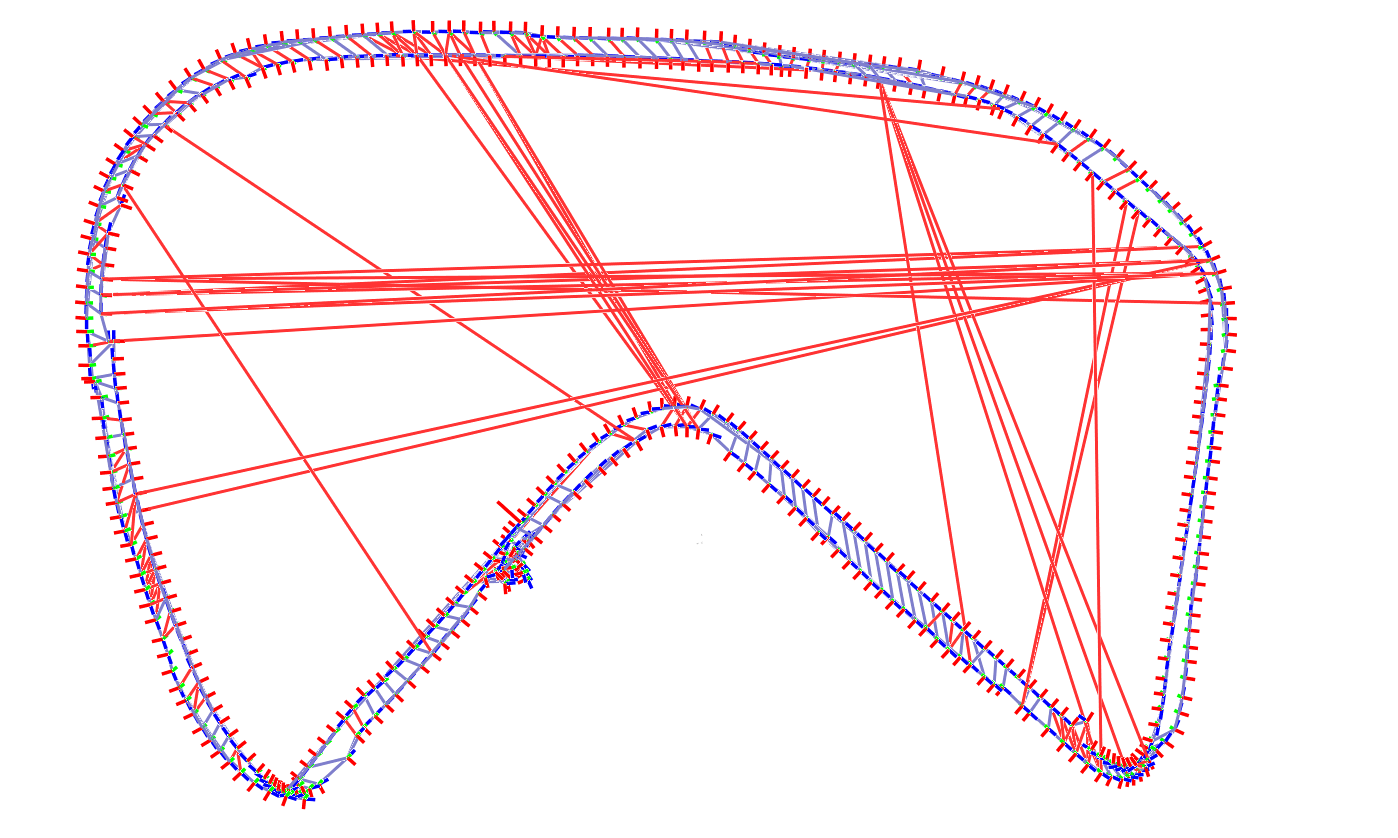
\includegraphics[width=0.32\textwidth]{chapters/images/half_fail}
    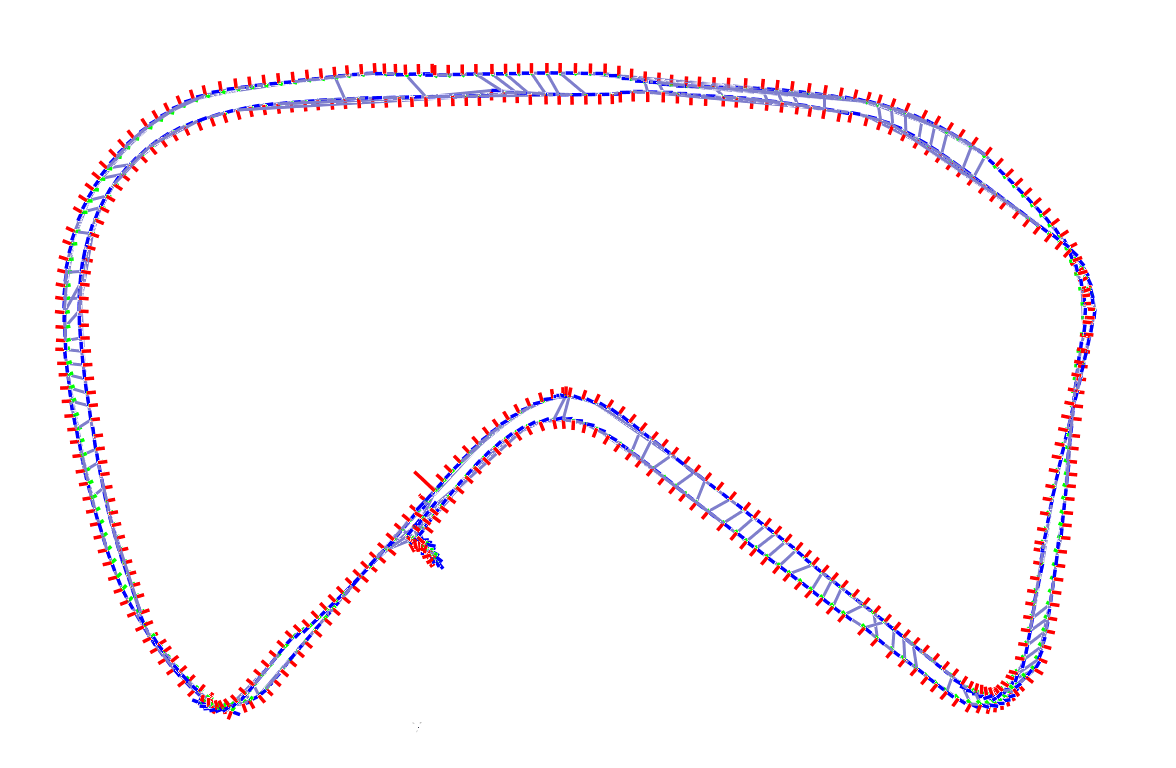
\includegraphics[width=0.32\textwidth]{chapters/images/omni_above}
  \caption{Different levels of loop closure filtering.  Left shows all loop closures generated from the place recognition module.  Center shows keyframes with matches and Right shows only successful omni-loop-closures}
  \label{fig:place_recog_stats}
\end{figure}

\subsection{Performance impact}

This section will briefly discuss the processing time omni-loop-closure pipeline and its impact on ScaViSLAM system.

\begin{table}[h]
  \centering
    \begin{tabular}{ p{5cm} r r} % p{5cm} |}
    \toprule
     & Features Cached & Features not caches \\
    \midrule
    Successful Loop closure   & 214ms & 735ms \\
    Unsuccessful loop closure & 58ms  & 564ms \\
    \bottomrule
    \end{tabular}
    \captionof{table}{Average computation times for the omni-loop-closure pipeline}
  \label{tab:timing_results}
\end{table}

Table \ref{tab:timing_results} shows computation time for the pipeline.  SIFT features are cached for keyframes which have been processed before, to avoid repetition of heavy computation.  Given that keyframes would be typically added at a rate of 0.5-1Hz based on parameters and scene, this imposes a very low impact on the ScaViSLAM system.  In addition the pipeline runs in a different thread to ScaViSLAM.

The time required for a failure case is also very important.  As shown above, the place recognizer produced many false positives.  In order to deal with this, more results from the place recognizer were taken and filtered by the geometry check.  However in order to do more geometry checks, it is important that it fails early on a false positive.  Less than 60ms allows many keyframe pairs to be tested for each new keyframe added.

Fig \ref{fig:pie_graph} shows the timing breakdown for a successful loop closure.  Most of the time is consumed either matching between omni camera frames or circular matching frame.  A potential improvement to this would be to do circular matching and scale offset calculation from source and target frames in parallel.  Another improvement would be to calculate SIFT features for stereo images and omni camera image in parallel.  However this calculation is already taking place on the GPU, and if there is good GPU utilization for this calculation then little would be gained in parallelizing this process.


\begin{figure}[H]
  \centering
    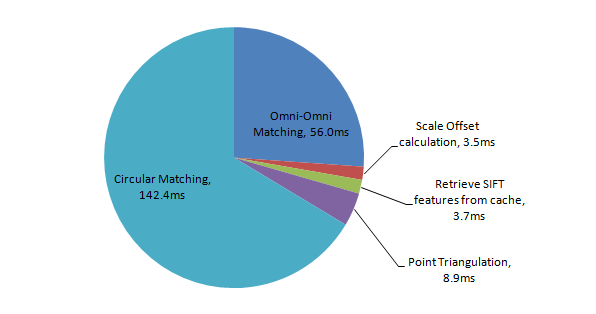
\includegraphics[width=0.7\textwidth]{chapters/images/pie_graph}
  \caption{Timing breakdown for a successful loop closure}
  \label{fig:pie_graph}
\end{figure}